\documentclass[10pt]{article}
\usepackage{icmlko}

\icmlmeta{IP 파운데이션 월드모델}{282}{내가 만든 문}{잎 하한을 정식으로 판정했더니 규칙이 통과시켰다 --- 그리고 그 규칙에 구멍이 있다는 것도 같이 나왔다}

\begin{document}

\twocolumn[
\icmlheader

\begin{abstract}
노트 276이 잎 하한을 5로 내리면 팝업이 라벨 누출 열로 $+$0.4373 을 얻는 것을
보였다. 그건 진단이었다. 이번엔 \textbf{진짜 축 스물셋}에서 누출 없이 잎
하한만 바꿔 노트 275의 규칙으로 정식 판정했다. \textbf{판은 셋 다 미결정 폭
안이다} --- 0.4857(20) · 0.4840(10) · 0.4849(5), 최대 폭 0.0017 로 노트 245의
0.010 의 6분의 1 이다. 규칙 ②(어느 도메인도 $|t|{>}2$ 로 안 나빠질 것)에서
갈렸다: \textbf{20$\to$10 은 도서 $-$0.0644($t{=}{-}2.24$)로 탈락},
\textbf{20$\to$5 는 제일 나쁜 것이 팝업 $-$0.0253($t{=}{-}1.11$)로 통과}
(\texttt{spread} 진짜 0개). \textbf{그런데 여기서 내가 쓴 규칙의 구멍이
보인다.} 도메인이 아홉이면 귀무 아래서도 $|t|{>}2$ 가 적어도 하나 나올
확률이 \textbf{34\%}(기대 개수 0.41)다. 도서의 $-$2.24가 정확히 그 크기이고,
같은 비교에서 웹툰이 $+$2.4 로 반대편에 있다 --- \textbf{둘 다 우연으로 설명이
된다.} 아홉 도메인 본페로니 문턱은 $|t|{>}2.77$ 이고 그러면 둘 다 유의하지
않다. \textbf{규칙 ②를 고친다: 문턱을 도메인 수에 맞춘다.} 그리고 결론은
\textbf{잎 하한을 안 바꾼다} --- 규칙 ①②를 통과했어도 노트 275의 규칙은
``통과하면 \emph{배포 이득이} 정한다''이지 ``통과하면 바꾼다''가 아니고,
노트 277이 확인한 대로 \textbf{지금 팝업에 쓸 전용 정보가 없다}. \textbf{문이
열렸는데 들어갈 것이 없다.}
\end{abstract}
]

\section{진단이 아니라 판정으로}

노트 276이 잎 하한을 20 $\to$ 10 $\to$ 5 로 내리며 팝업의 라벨 누출 열이
$+$0.0000 $\to$ $+$0.0394 $\to$ $+$0.4373 으로 살아나는 것을 보였다.
\textbf{그 판에는 누출 열이 들어 있었다} --- 기전을 보려고 만든 것이지
쓰겠다는 게 아니다.

정식 판정은 다르다. \textbf{지금 쓰는 축 스물셋 그대로}, 누출 없이, 문턱 15
에서 잎 하한만 바꾼다. 그리고 노트 275가 세운 규칙에 건다.

\begin{quote}\small
어떤 변경이 \textbf{①} 판에서 미결정 폭 안이고 \textbf{②} 어느 도메인에서도
$|t|{>}2$ 로 나빠지지 않으면, 배포 쪽 이득이 정한다.
\end{quote}

\section{판은 움직이지 않는다}

\begin{figure*}[t]
\centering
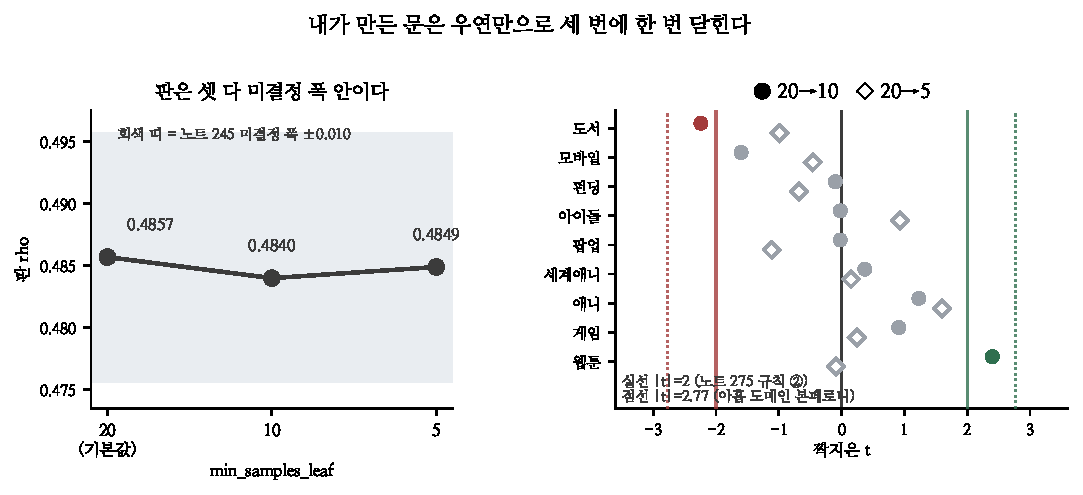
\includegraphics[width=\textwidth]{figs/gate.pdf}
\caption{왼쪽 --- 잎 하한별 판 $\rho$. 회색 띠가 노트 245의 미결정 폭
$\pm$0.010. 오른쪽 --- 도메인별 짝지은 $t$. 실선이 노트 275 규칙 ②의
$|t|{=}2$, 점선이 아홉 도메인 본페로니 $|t|{=}2.77$.}
\end{figure*}

\begin{center}\small
\begin{tabular}{rrrrrr}
\hline
잎 하한 & 판 & 팝업 & 아이돌 & 펀딩 & 도서 \\
\hline
20 & 0.4857 & 0.3931 & 0.1289 & 0.2580 & 0.3773 \\
10 & 0.4840 & 0.3927 & 0.1282 & 0.2564 & 0.3129 \\
5 & 0.4849 & 0.3678 & 0.1940 & 0.2475 & 0.3510 \\
\hline
\end{tabular}
\end{center}

\textbf{판의 최대 폭이 0.0017 이다} --- 미결정 폭의 6분의 1. 규칙 ①은 둘 다
통과다. 그리고 \textbf{단조도 아니다}(10이 20과 5보다 낮다) --- 손잡이가
평평하다는 또 하나의 신호고, 이 실험실이 알파 · $\tau$ · 깊이에 이어 네
번째로 만나는 모양이다.

\section{규칙 ②에서 갈렸다 --- 그리고 그 규칙이 샌다}

\begin{center}\small
\begin{tabular}{lrrr}
\hline
20 $\to$ 10 & 차 & 짝SE & $t$ \\
\hline
\textbf{도서} & \textbf{$-$0.0644} & 0.0288 & \textbf{$-$2.24} \\
모바일 & $-$0.0033 & 0.0021 & $-$1.60 \\
$\cdots$ & & & \\
\textbf{웹툰} & \textbf{$+$0.0065} & 0.0027 & \textbf{$+$2.40} \\
\hline
\multicolumn{4}{l}{판 $-$0.0017 · 진짜 총량 0.0058 · 진짜 2개} \\
\hline
20 $\to$ 5 & & & \\
\hline
도서 & $-$0.0263 & 0.0267 & $-$0.99 \\
팝업 & $-$0.0253 & 0.0227 & $-$1.11 \\
아이돌 & $+$0.0651 & 0.0697 & $+$0.93 \\
\hline
\multicolumn{4}{l}{판 $-$0.0008 · 진짜 총량 0.0000 · \textbf{진짜 0개}} \\
\hline
\end{tabular}
\end{center}

규칙대로면 \textbf{20$\to$10 탈락}(도서 $-$2.24), \textbf{20$\to$5 통과}다.

\paragraph{그런데 도메인이 아홉이다} 규칙 ②는 아홉 개를 동시에 본다. 귀무
아래에서 한 도메인이 $|t|{>}2$ 일 확률이 0.0455 이니 \textbf{적어도 하나
나올 확률이 34\%}이고 기대 개수가 0.41 이다.

\begin{center}\small
\begin{tabular}{lr}
\hline
아홉 도메인 · $|t|{>}2$ 문턱 & \\
\hline
한 도메인 우연 확률 & 0.0455 \\
\textbf{적어도 하나 나올 확률} & \textbf{34.2\%} \\
기대 개수 & 0.41 \\
본페로니 문턱 & $|t| > 2.77$ \\
\hline
\end{tabular}
\end{center}

\textbf{도서의 $-$2.24가 정확히 그 크기다.} 그리고 같은 비교에서 웹툰이
$+$2.40 으로 반대편에 있다 --- 손해 하나와 이득 하나가 대칭으로 나온 것은
잡음의 모양이지 효과의 모양이 아니다. 본페로니 문턱 2.77 로 보면 \textbf{둘
다 유의하지 않고}, 20$\to$10 도 통과가 된다.

\paragraph{규칙을 고친다} 노트 275에서 ``$|t|{>}2$''라고 쓴 것은 노트 248이
도메인별 수를 SE 와 함께 읽으라고 한 데서 왔는데, \textbf{한 도메인을 볼
때의 문턱을 아홉 개에 그대로 썼다.} 고친 형태는 이렇다.

\begin{quote}\small
\textbf{②} 어느 도메인에서도 $|t| > z(0.05/2K)$ 로 나빠지지 않을 것
($K$ 는 채점 도메인 수 --- 지금 아홉이면 2.77).
\end{quote}

이 실험실이 같은 함정에 이미 한 번 빠졌다 --- 더현대 ``22$\sim$47\%'' 진술이
체리피킹이었고, 그때 세운 규약이 ``부분집합 주장엔 반드시 제외 기준 명시''
였다. \textbf{이번 것은 그 짝이다: 여럿을 동시에 볼 때는 문턱을 올린다.}

\section{그래서 안 바꾼다}

규칙 ①②를 20$\to$5 가 통과했고, 고친 규칙으로는 20$\to$10 도 통과한다.
\textbf{그래도 안 바꾼다.}

노트 275의 규칙은 ``통과하면 바꾼다''가 아니라 \textbf{``통과하면 배포
이득이 정한다''}이다. 그러니 배포 이득이 있어야 한다. 그런데 노트 277이
확인했다 --- 팝업 전용 축 넷은 \textbf{능형에서도} $-$0.0070 이다. 즉 잎
하한을 내려 나무의 귀를 열어 줘도 \textbf{들려줄 말이 없다.}

\textbf{문이 열렸는데 들어갈 것이 없다.} 잎 하한은 이제 ``평평한 손잡이''가
아니라 \textbf{``조건부로 열려 있는 손잡이''}로 기록한다 --- 얇은 도메인의
쓸 만한 전용 축이 생기는 날, 이 문은 이미 판정을 통과해 있다.

\paragraph{덤 --- 아이돌 $+$0.0651} 20$\to$5 에서 제일 크게 오른 것이
아이돌이다($t{=}0.93$, 짝SE 0.0697 로 판에서 제일 나쁘다). 유의하지 않지만
방향이 이 노트들의 이야기와 맞는다 --- 아이돌은 학습 54행으로 벼랑 바로
위이고, 잎을 내리면 제 구조를 더 쓸 수 있다. \textbf{2호 도메인이 아이돌이니
이 수는 다시 볼 자리에 있다.}

\paragraph{남은 것}
\begin{center}\small
\begin{tabular}{ll}
\hline
갈래 & 왜 \\
\hline
규칙 ② 코드화 & \texttt{rank.spread} 가 $K$ 를 알고 문턱을 정하게 \\
아이돌 $+$0.0651 & 반복 씨앗으로 다시. 짝SE 0.07 이 벽 \\
진짜 축이 먼저 & 문보다 들어갈 것이 없는 게 문제다 \\
지난 판정 재검토 & $|t|{>}2$ 로 내린 결정이 또 있나 \\
\hline
\end{tabular}
\end{center}

\paragraph{규약} \textbf{규칙을 세울 때 그 규칙을 몇 번 적용하는지 센다.}
노트 275가 ``$|t|{>}2$''를 쓸 때 한 도메인을 생각했는데 실제로는 아홉에
동시에 걸린다 --- 우연만으로 세 번에 한 번 닫히는 문이었다. 그리고
\textbf{내가 만든 규칙도 통제 대상이다} --- 이 세션에서 내 주장이 좁혀진
다섯 번째이고, 앞의 넷은 측정이었지만 이번 것은 \textbf{판정 규칙 자체}였다.

\end{document}
